\section{Выбор модели классификации временных рядов}
Рассматривалась задача выбора модели классификации временных рядов.
В качестве промежуточного этапа производился выбор автокодировщика, чьи параметры оптимизировались без учителя. 
Модели автокодировщика имели вид
\[
    \mathbf{f}(\mathbf{x}, \mathbf{w}) = \mathbf{f}_\text{enc} \circ \mathbf{f}_\text{dec}(\mathbf{x}),
\]
где $ \mathbf{f}_\text{enc},  \mathbf{f}_\text{dec}$ --- подмодели автокодировщика, называемые кодером и декодером соответственно. Каждая из подмоделей имеет вид ограниченной машины Больцмана~\cite{hinton_rbm} с двумя скрытыми слоями.

На основе прооптимизированных моделей автокодировщиков проиходила оптимизация моделей классификации~\cite{finetuning}.
В качестве данных для проведения вычислительного эксперимента использовались данные WISDM~\cite{wisdm}, представляющие собой набор записей акселерометра мобильного телефона. Каждой записи соответствуют три координаты по осям акселерометра. Набор данных содержит записи движений для 6 классов переменной длины.
При проведении вычислительного эксперимента из каждой записи использовались первые 200 сегментов. Т. к. выборка не сбалансирована, в нее добавлялись повторы записей классов, содержащих количество записей, меньшее чем у большего класса.

Основные эксперименты --- исследование зависимости ошибки классификации от числа параметров и размера выборки --- были проведены как с использованием инструментария на базе библиотеки Theano, так и с использованием инструментария на языке Matlab.
Для оценки качества классификации была проведена процедура скользящего контроля~\cite{cv_ms} при соотношении числа объектов обучающей и контрольной выборки 3:1. Число нейронов на каждом слое задавалось из соотношения 10:6:3. При проведении процедуры скользящего контроля для каждого отсчета количества нейронов было произведено пять запусков. В эксперименте с использованием инструментария на базе Theano при обучении двухслойной нейронной сети проводился мультистарт~\cite{multi}, т.~е. одновременный запуск обучения сети с 8 разными стартовыми значениями параметров для предотвращения возможного застревания алгоритма обучения в локальном минимуме. При оценке качества классификации выбиралась модель с наилучшими результатами. График зависимости ошибки классификации от числа используемых нейронов изображен на рис.~\ref{fig:neurons}.



\begin{figure}[tb!]
 \centering
  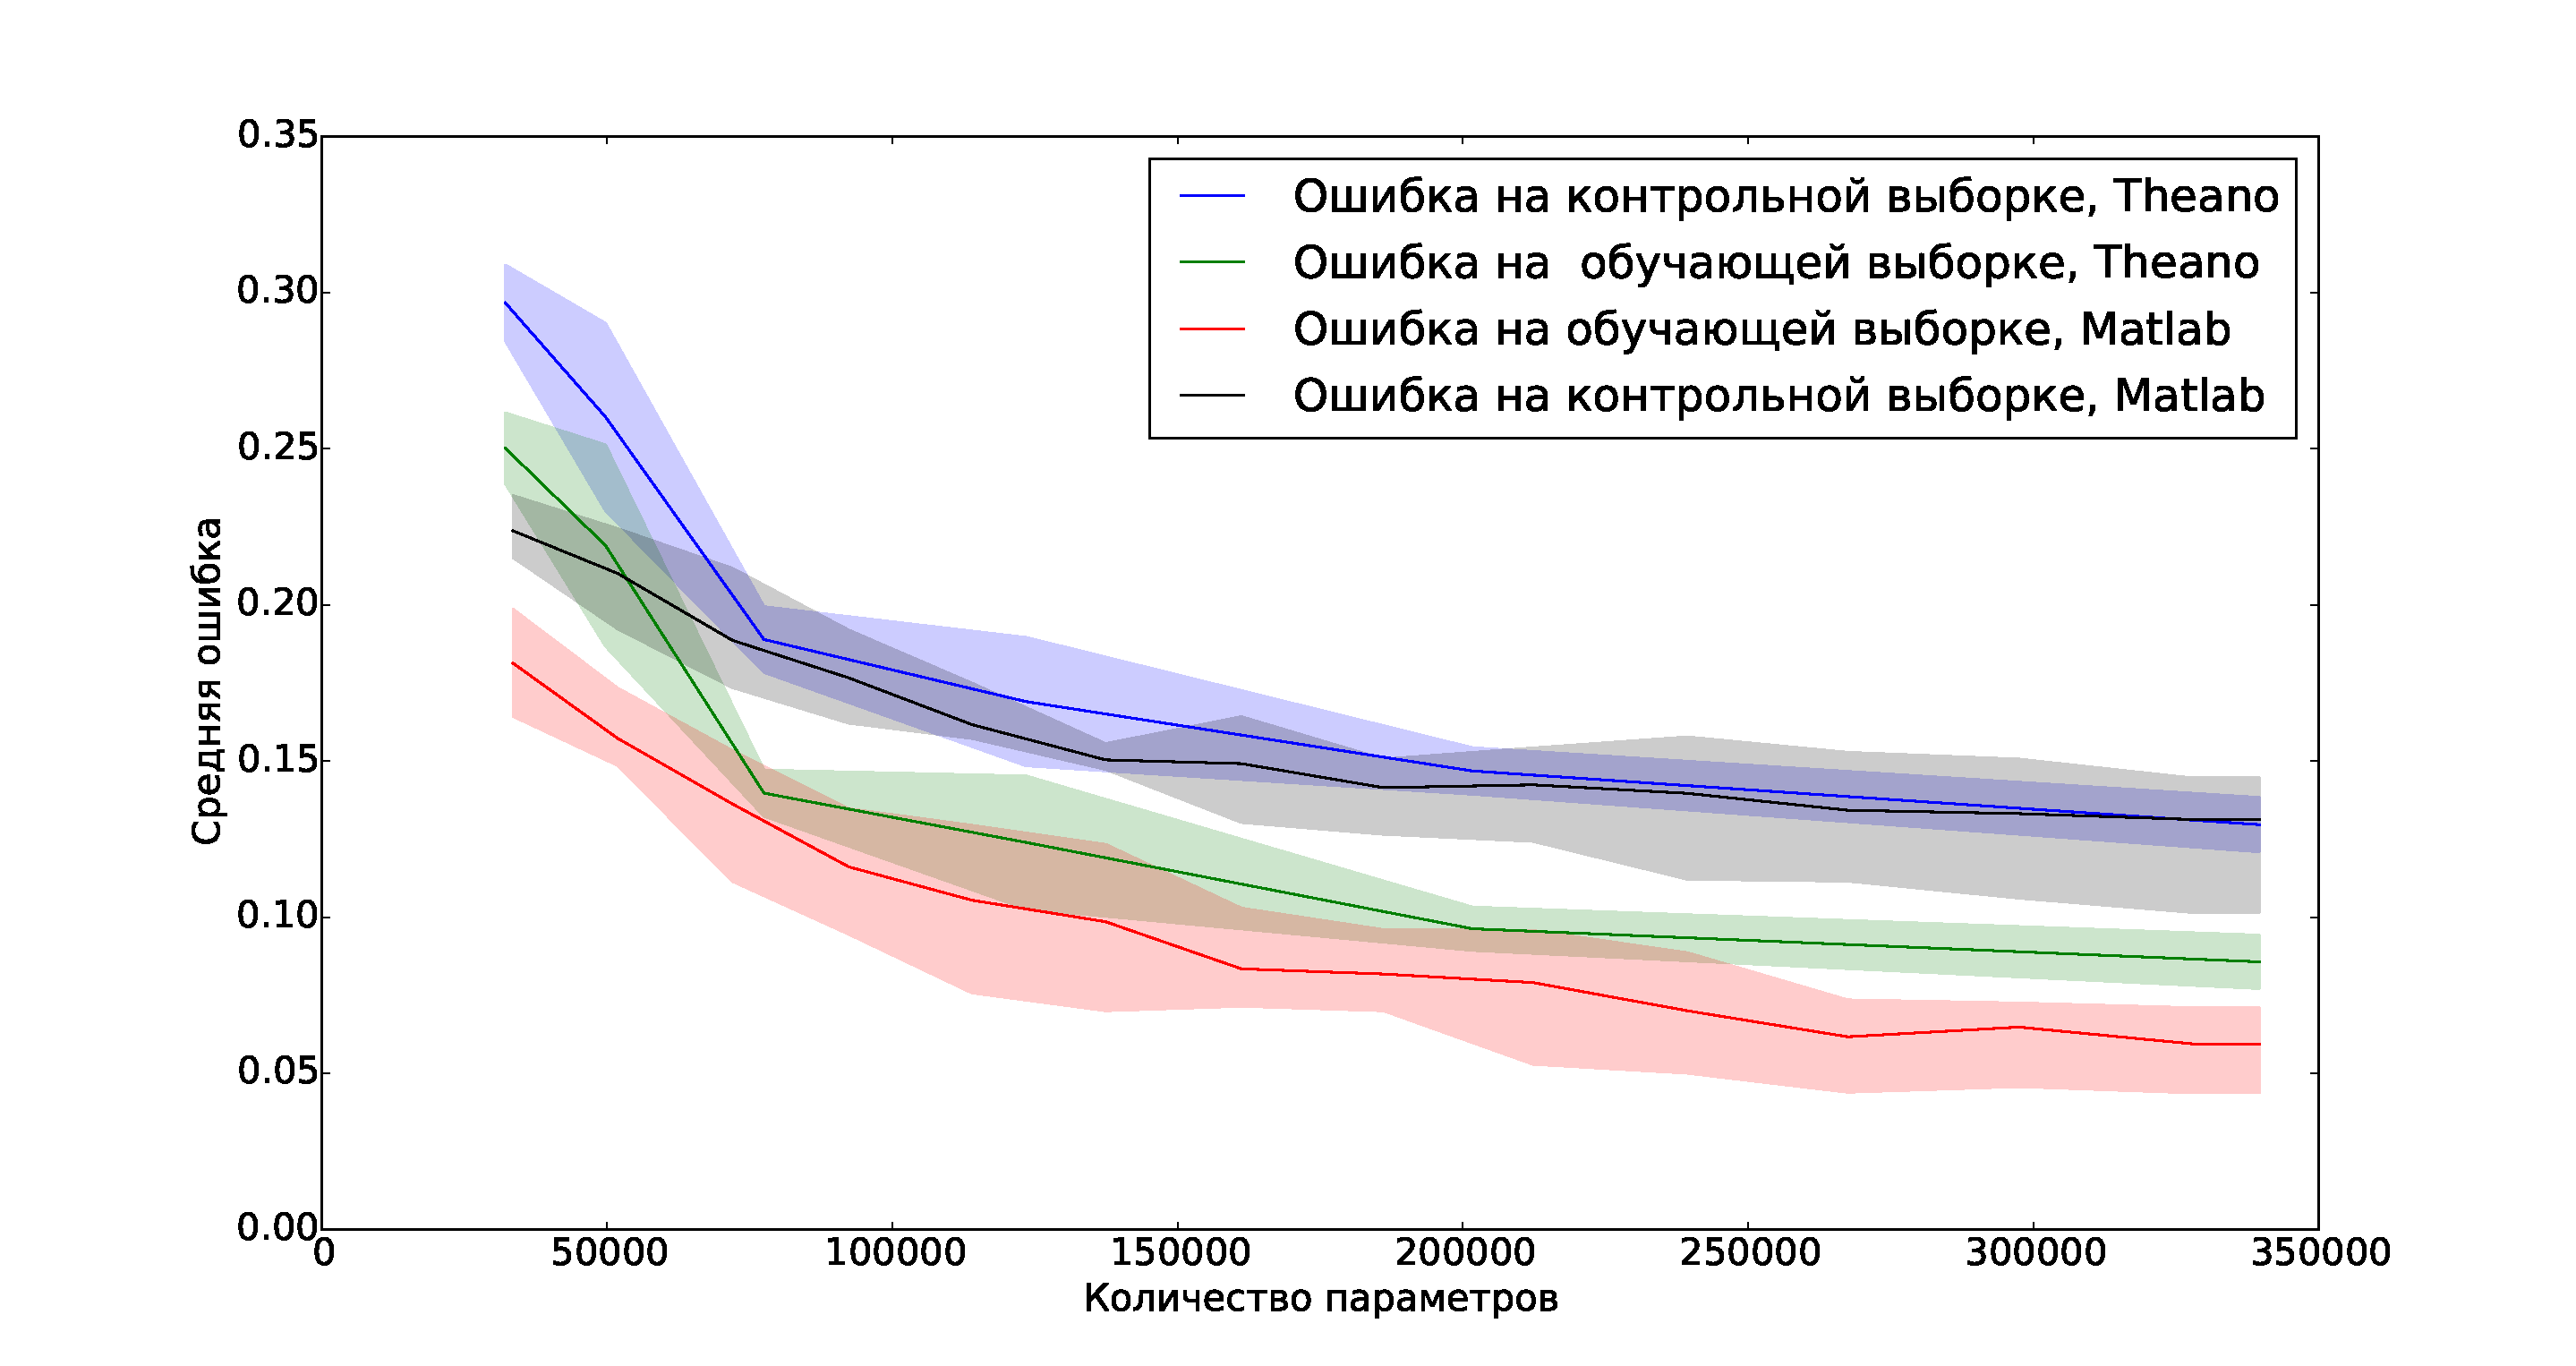
\includegraphics[width=1.0\textwidth]{plots/popova/neurons.pdf}
 \caption{Зависимость ошибки     от числа нейронов}
 \label{fig:neurons}
\end{figure}


Для оценки зависимости качества классификации от размера обучающей выборки была проведена кроссвалидация с фиксированным количеством объектов в обучающей выборке (25\% исходной выборки) и переменным размером обучающей выборки. Число нейронов было установлено как 364:224:112. При проведении процедуры скользящего контроля для каждого отсчета было произведено пять запусков. График зависимости ошибки классификации от размера обучающей выборки представлен на рис.~\ref{fig:samples}.


\begin{figure}[tb!]
 \centering
  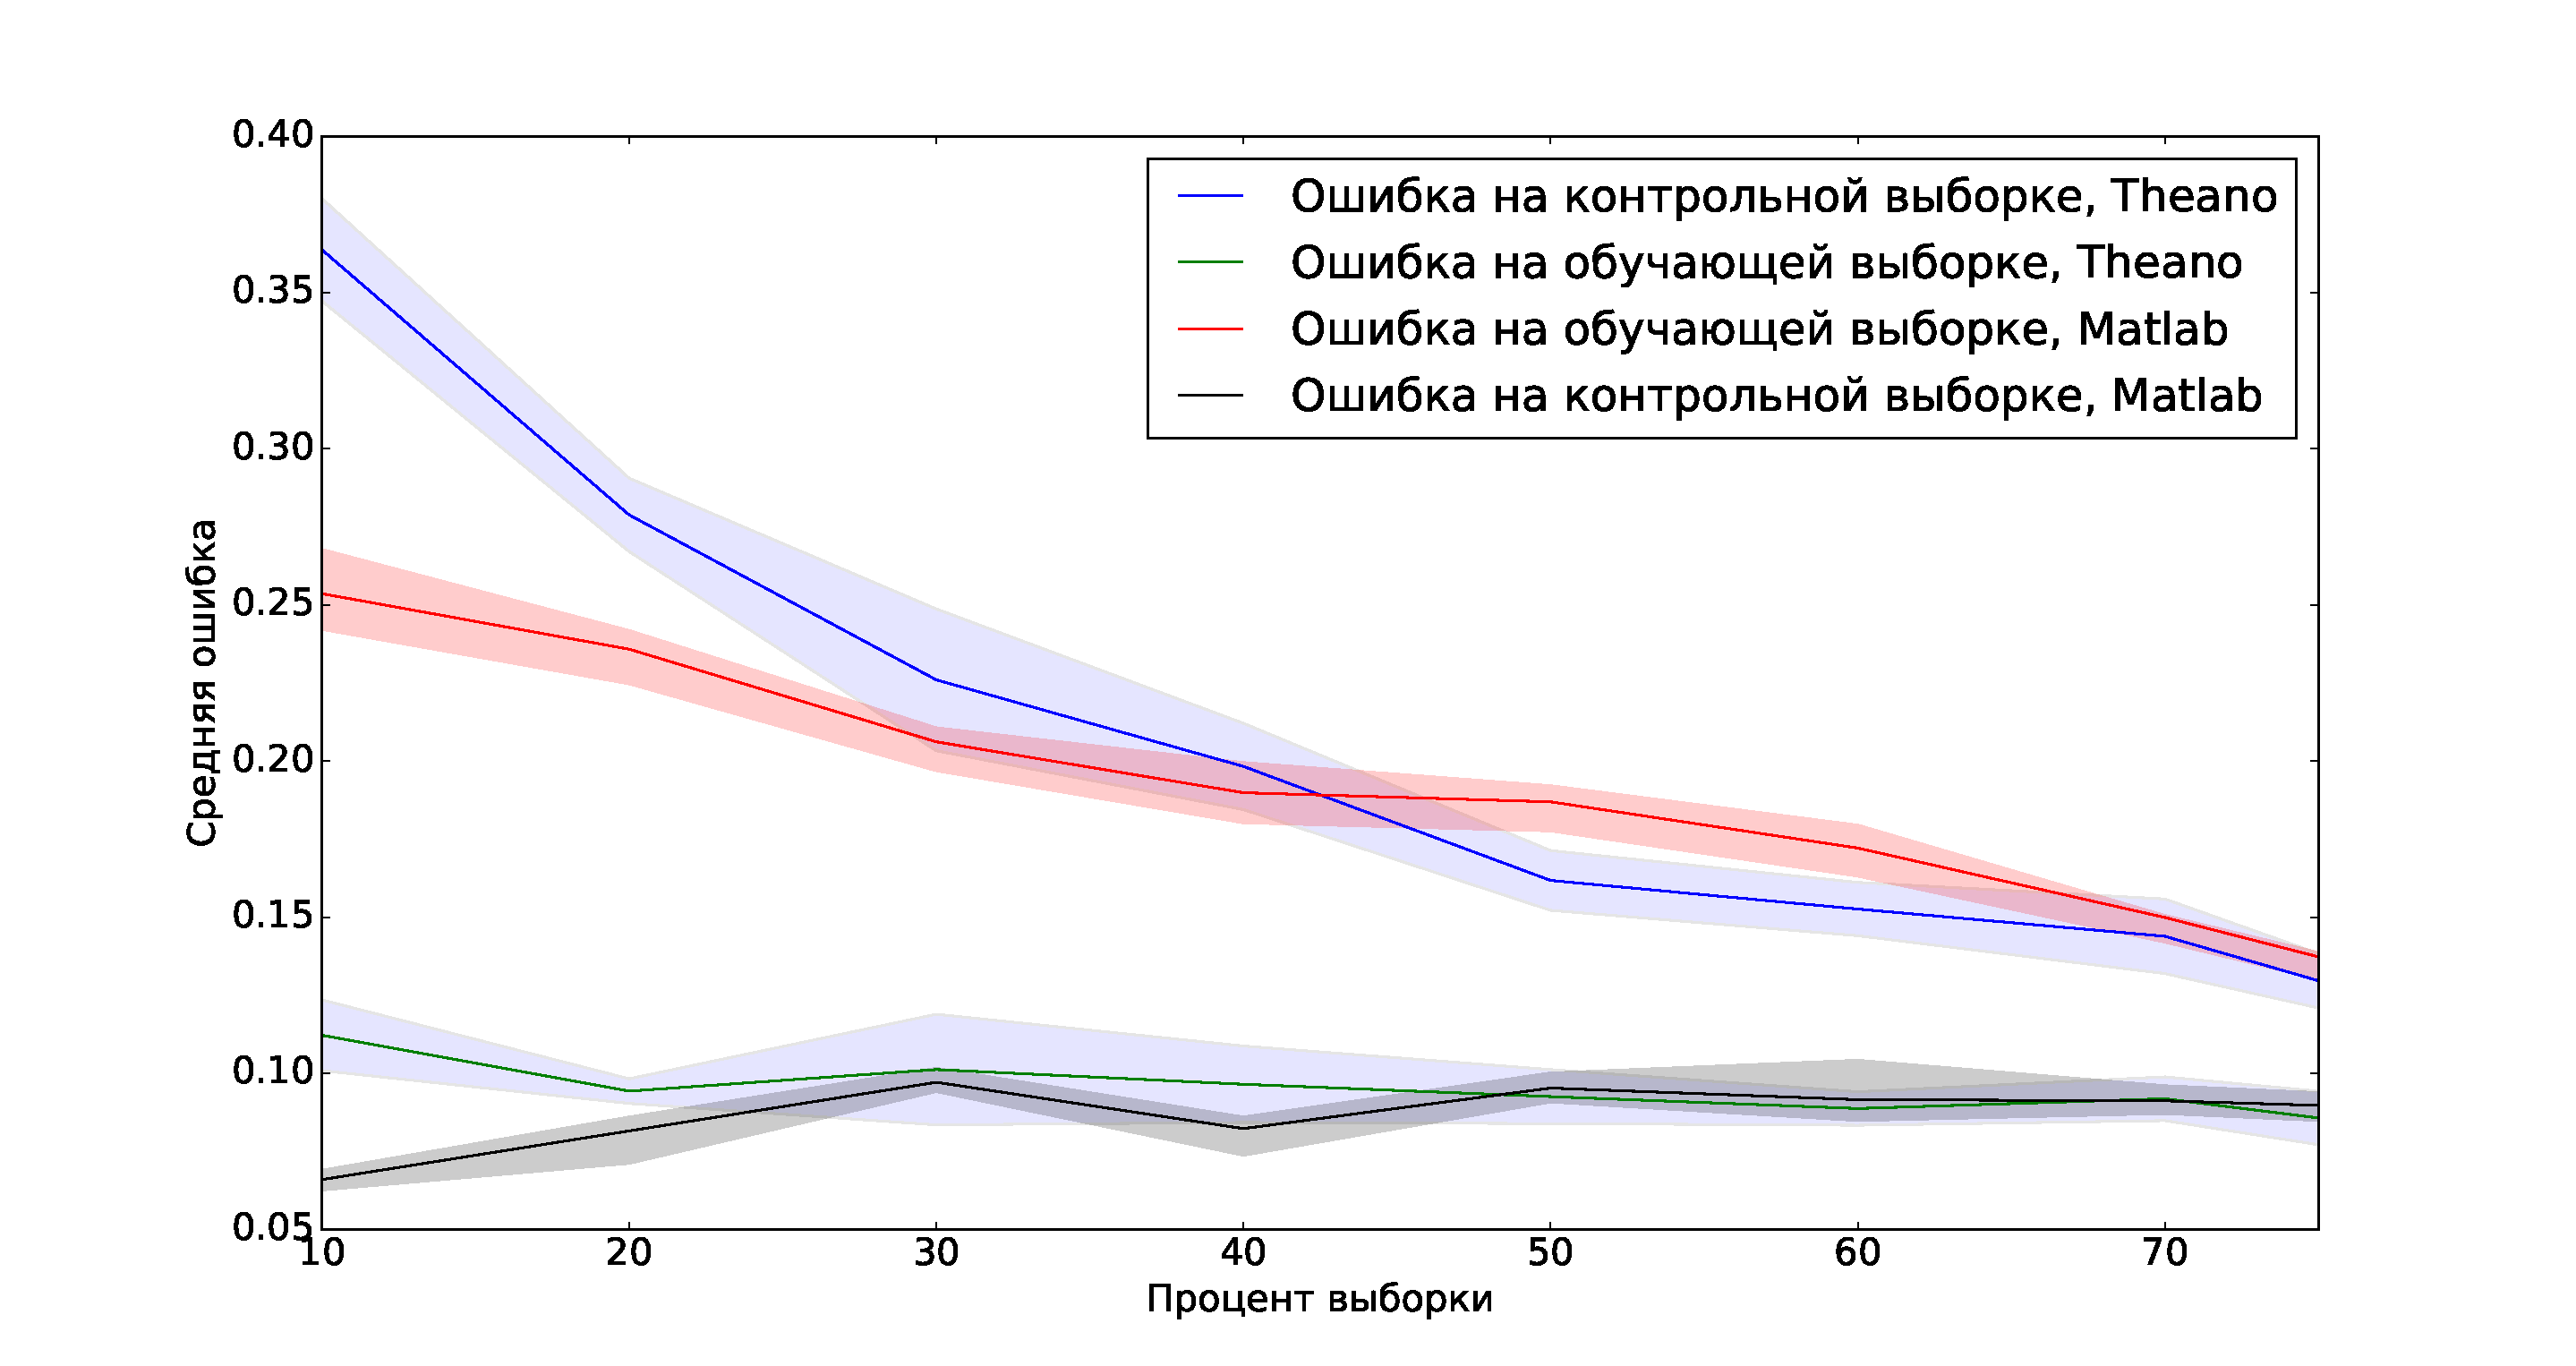
\includegraphics[width=1.0\textwidth]{plots/popova/samples.pdf}
 \caption{Зависимость ошибки от размера обучающей выборки}
 \label{fig:samples}
\end{figure}


Для исследования скорости работы процесса обучения нейросети в зависимости от конфигурации Theano был сделан следующий эксперимент:
проводилось обучение двухслойной нейросети на основе подсчитанных заранее параметров ограниченной машины Больцмана~\eqref{eq:rbm} и автокодировщика~\eqref{eq:ae}. Обучение проходило за 100 итераций. При обучении алгоритм запускался параллельно с $n$ разными стартовыми позициями, $n \in \{1,\dots,4\}.$ Число нейронов было установлено как 300:200:100.
Запуск осуществлялся со следующими конфигурациями Theano:
\begin{itemize}
\item вычисление на центральном процессоре, задействовано
одно ядро;
\item вычисление на центральном процессоре, задействовано четыре ядра;
\item вычисление на центральном процессоре, задействовано восемь ядер;
\item вычисление на графическом процессоре.
\end{itemize}

Результаты эксперимента приведены на рис.~\ref{fig:speed}. Как видно из графика, вычисление с использованием CUDA показывает значительное ускорение по сравнению с вычислением на центральном процессоре.

\begin{figure}[tb!]
 \centering
  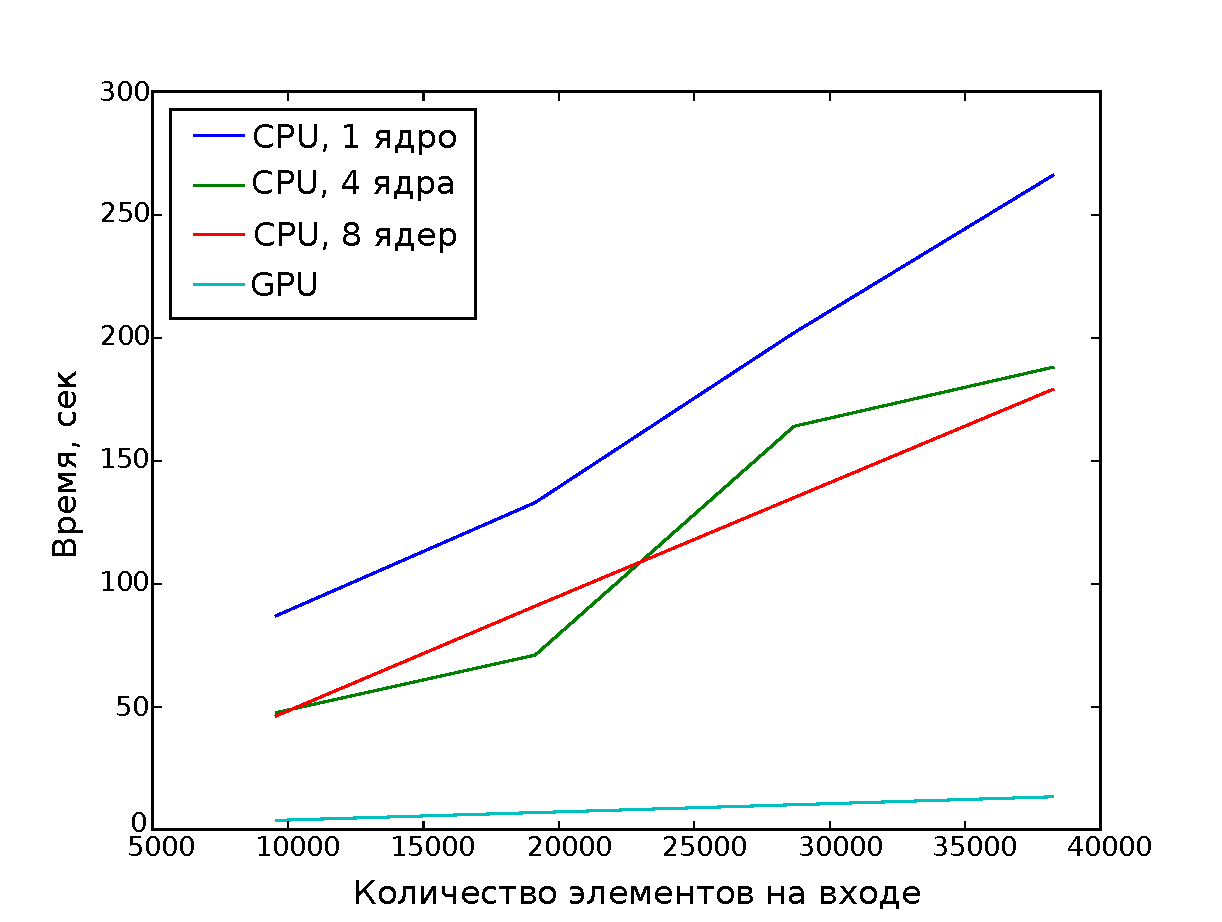
\includegraphics[width=0.8\textwidth]{plots/popova/result.pdf}
 \caption{Результаты эксперимента по исследованию скорости процесса обучения}
 \label{fig:speed}
\end{figure}




\section{Модели парафраза (Смердов)}
Цель эксперимента~--- проверка работоспособности предложенного алгоритма и сравнение результатов с ранее полученными. В качестве данных использовалась выборка SemEval 2015, состоящая из 8331 пары схожих и несхожих предложений. Слова преобразовывались в векторы размерности 50 при помощи алгоритма GloVe~\cite{GloveURL}.
%\footnote{https://github.com/stanfordnlp/GloVe}
Для базовых алгоритмов тренировочная, валидационная и тестовая выборки составили 70\%, 15\% и 15\% соответственно.
Для рекуррентной нейронной сети, полученной вариационным методом, валидационная выборка отсутствовала, а тренировочная и тестовая выборки составили 85\% и 15\% соответственно.
Критерием качества была выбрана F1-мера.
В качестве базовых алгоритмов использовались линейная регрессия, метод ближайших соседей, решающее дерево и модификация метода опорных векторов SVC. Базовые алгоритмы взяты из библиотеки sklearn. 
%\cite{sklearn}.
%\footnote{http://scikit-learn.org/stable/}.
Дополнительно были построены рекуррентная нейросеть с одним скрытым слоем~\cite{Sanborn} и нейросеть с одним скрытым слоем и вариационной оптимизацией параметров~\cite{Graves, code}.
% \footnote{https://sourceforge.net/p/mlalgorithms/code/HEAD/tree/Group474/Smerdov2017Paraphrase/code/}.

% Как показал вычислительный эксперимент, вариационная нейросеть, полученная методом, описанным в~\cite{Graves}, позволяет значительно улучшить качество предсказаний.
\begin{figure}[!h]
	\centering
	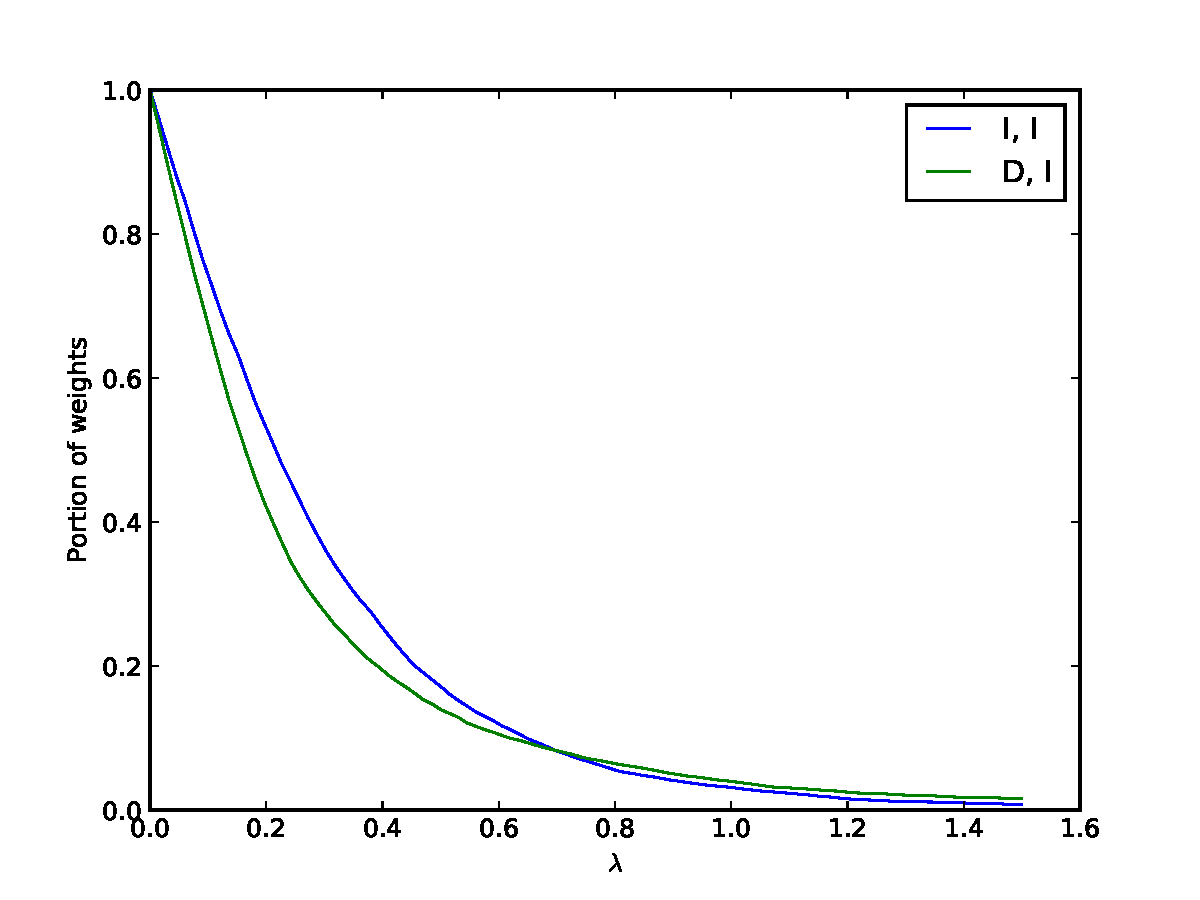
\includegraphics[width=0.5\textwidth]{plots/smerdov/lambdas.pdf}
	\caption{Доля неудаленных параметров сети в зависимости от порогового значения $\lambda$ для скалярного~($I$) и диагонального~($D$) вида апостериорной матрицы ковариаций}
	\label{lambdas}
\end{figure}

 

На рис.~\ref{evidence_I_I} и~\ref{evidence_I_D} представлена зависимость оценки правдоподобия $L$ \eqref{loss} от параметра $\lambda$.
%Видно, что существует некоторое оптимальное значения $\lambda$, при котором оценка минимальна --- именно это значение $\lambda$ соответствует оптимальной модели.
Для обоих случаев существует оптимальное значение $\lambda$, минимизирующее $L$; модели с таким параметром будут оптимальными. На рис.~\ref{score_I_I},~\ref{score_I_D},~\ref{portion_I_I} и~\ref{portion_I_D} отображены зависимости качества модели от $\lambda$ и доли выброшенных параметров. Видно, что даже при удалении большинства параметров из сети качество предсказаний меняется несущественно, что говорит о слишком большом числе параметров исходной модели.

Из рис.~\ref{lambdas} видно, что при малых $\lambda$ из сети с диагональной апостериорной матрицей ковариаций удаляется больше весов, а при больших $\lambda$ --- меньше, что говорит о лучшем отборе параметров такой моделью.


\section{Прореживание модели (Грабовой)}
Для анализа свойств предложенного алгоритма и сравнения его с существующими был проведен вычислительный эксперимент в котором параметры нейросети удалялись методами,  которые были описаны в разделах 3.1---3.3 и методом Белсли.

В качестве данных использовались три выборки. Выборки Wine~\cite{Wine} и Boston~Housing~\cite{Boston}  --- это реальные данные. Синтетические данные сгенерированы таким образом чтобы параметры сети были мультиколинеарными. Генерация данных состояла из двух этапов. 
На первом этапе генерировался вектор параметров $\mathbf{w}_{\text{synthetic}}$:
$$\mathbf{w}_{\text{synthetic}}  \sim \mathcal{N}(\textbf{m}_{\text{synthetic}}, \textbf{A}_{\text{synthetic}}), \eqno(5.1)$$ 
где 
$\textbf{m}_{\text{synthetic}} = \begin{bmatrix}
1.0\\
0.0025\\
\cdots\\
0.0025
\end{bmatrix}$,
$\textbf{A}_{\text{synthetic}} = \begin{bmatrix}
1.0& 10^{-3}& \cdots& 10^{-3}& 10^{-3}\\
10^{-3}& 1.0& \cdots& 0.95& 0.95\\
\cdots&\cdots&\cdots&\cdots&\cdots\\
10^{-3}& 0.95& \cdots& 0.95& 1.0
\end{bmatrix}$.

На втором этапе генерировалась выборка $\mathfrak{D}_{\text{synthetic}}$:
$$\mathfrak{D}_{\text{synthetic}} = \{(\textbf{x}_i,y_i)| \textbf{x}_i \sim  \mathcal{N}(\textbf{1}, \textbf{I}), y_i = x_{i0}, i = 1 \cdots 10000\}. \eqno(5.2)$$
В приведенном выше векторе параметров $\mathbf{w}_{\text{synthetic}}$ для выборки $\mathfrak{D}_{\text{synthetic}}$, наиболее релевантным является первый параметр, а все остальные параметры являются нерелевантными. Матрица ковариации была выбрана таким образом, чтобы все нерелевантные параметры были зависимы и метод Белсли был максимально эффективен.



\begin{table}[h]

\begin{center}
\caption{Описание выборок}
\begin{tabular}{|c|c|c|c|}
\hline
	Выборка &Тип задачи& Размер выборки& Число признаков\\
	\hline
	
	\multicolumn{1}{|l|}{Wine}
	&
	\multicolumn{1}{|l|}{класификация}
	 & 178 & 13\\
	\hline
	
	\multicolumn{1}{|l|}{Boston Housing}
	&
	\multicolumn{1}{|l|}{регресия}
	& 506 & 13\\
	\hline
	
	\multicolumn{1}{|l|}{Synthetic data}
	&
	\multicolumn{1}{|l|}{регресия}
	& 10000 & 100\\
\hline

\end{tabular}
\end{center}
\end{table}



Для алгоритмов тренировочная и тестовая выборки составили~$80\%$ и~$20\%$ соответсвенно. Критерием качества прореживания служит процент параметров нейросети, удаление которого не влечет значимой потери качества прогноза. Также критерием качества служит устойчивость нейросети к зашумленности данных. 

Качеством прогноза $R_{\text{cl}}$ модели для задачи классификации является точность прогноза модели:
$$R_{\text{cl}} = \frac{\sum_{(\textbf{x},y)\in \mathfrak{D}} [f(\textbf{x}, \textbf{w}) = y]}{\left|\mathfrak{D}\right|}, \eqno(5.3)$$

Качеством прогноза $R_{\text{rg}} $ модели для задачи регрессии является среднеквадратическое отклонение результата модели от точного:

$$R_{\text{rg}} = \frac{\sum_{(\textbf{x},y)\in \mathfrak{D}} \left(f(\textbf{x}, \textbf{w}) - y\right)^2}{\left|\mathfrak{D}\right|}, \eqno(5.4)$$

\textbf{Wine.} Рассмотрим нейроную сеть с 13 нейронами на входе, 13 нейронами в скрытом слое и 3 нейронами на выходе.

\begin{figure}[h!t]\center
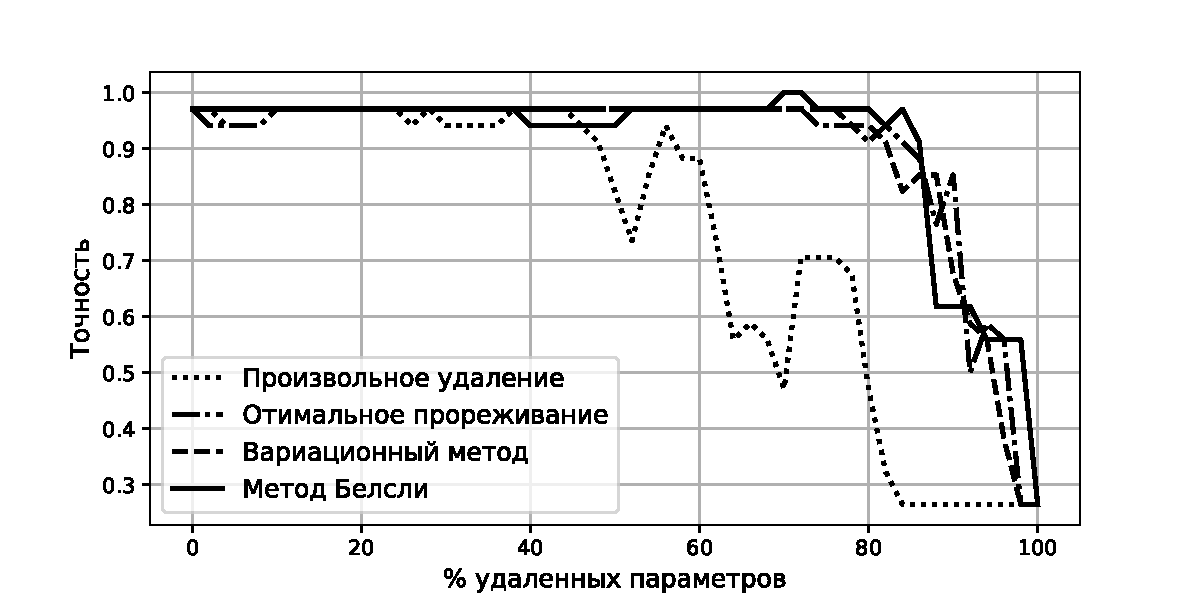
\includegraphics[width=0.8\textwidth]{plots/grabovoy/wine_all.pdf}\\
\caption{Качество прогноза при удаление параметров на выборке Wine}
\label{WineAll}
\end{figure}

\begin{figure}[ht]\center
%\begin{subfigure}[а]{0.33\textwidth}
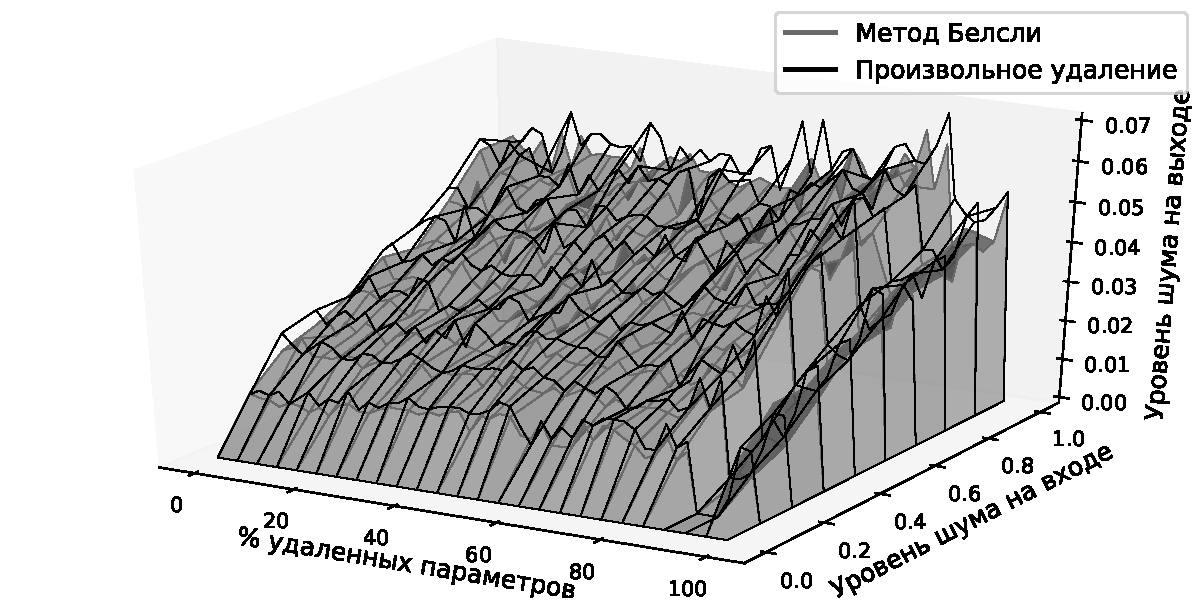
\includegraphics[width=0.33\textwidth]{plots/grabovoy/wine_random_noise3d.pdf}
%\end{subfigure}
%\begin{subfigure}[б]{0.33\textwidth}
{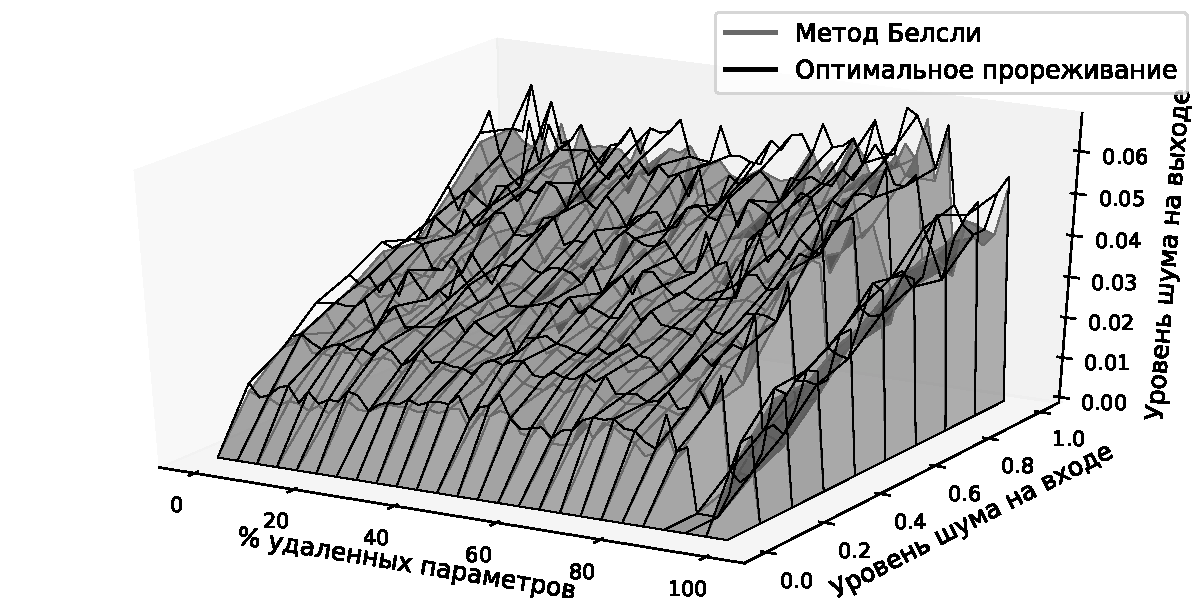
\includegraphics[width=0.33\textwidth]{plots/grabovoy/obd_noise_3d.pdf}}
%\end{subfigure}
%\begin{subfigure}[в]{0.33\textwidth}
{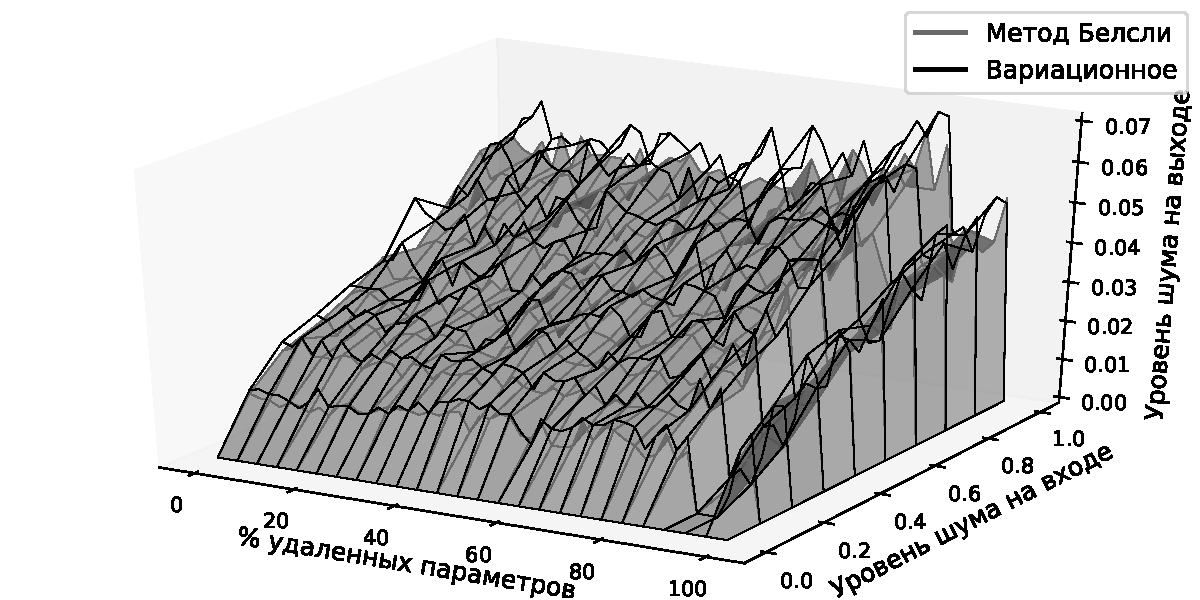
\includegraphics[width=0.33\textwidth]{plots/grabovoy/var_noise_3d.pdf}}
%\end{subfigure}

%\subfigure[Оптимальное прореживание]{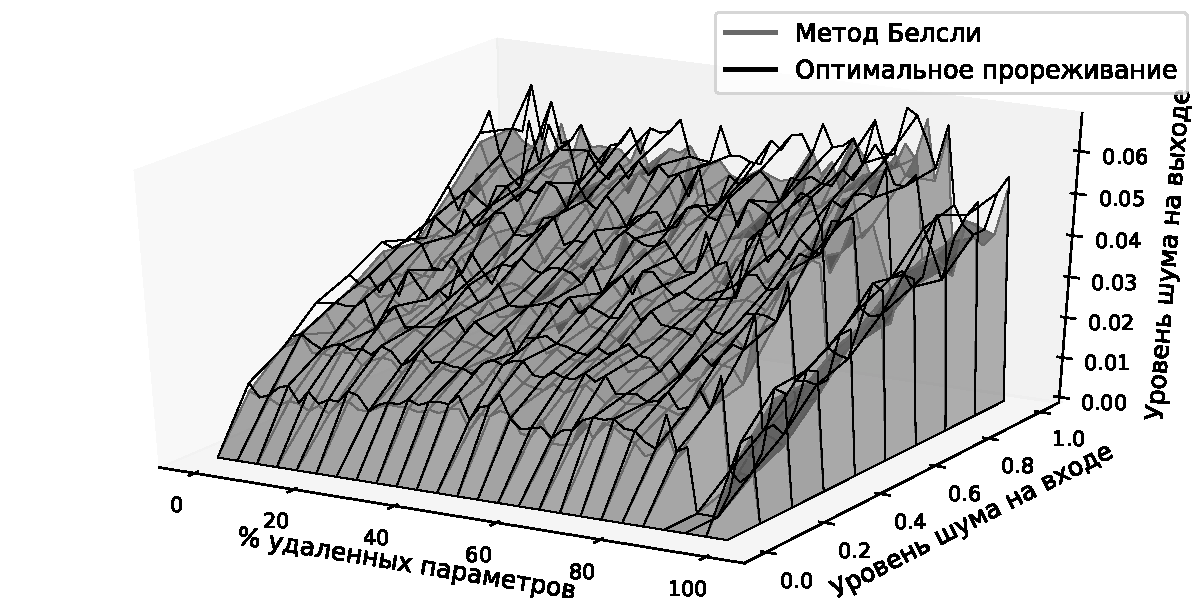
\includegraphics[width=0.5\textwidth]{plots/grabovoy/obd_noise_3d.pdf}}\\
%\subfigure[Вариационный метод]{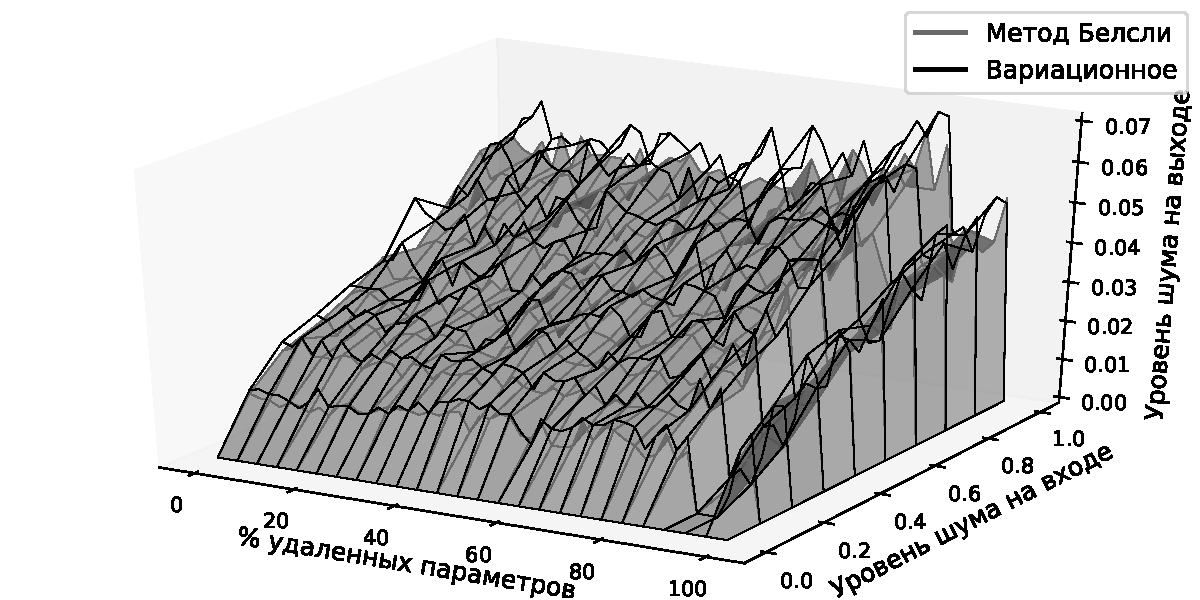
\includegraphics[width=0.5\textwidth]{plots/grabovoy/var_noise_3d.pdf}}
\caption{Влияние шума в начальных данных на шум выхода нейросети на выборке Wine: a --- Произвольное удаление параметров, б --- Оптимальное прореживание, в --- Вариационный метод}
\label{WineNoise}
\end{figure}

На рис.~\ref{WineAll} показано как меняется точность прогноза $R_{\text{cl}}$ при удалении параметров указанными методами. Из графика видно, что метод оптимального прореживания, вариационный метод и метод Белсли позволяют удалить $\approx80\%$ параметров и качество всех этих методов падает при удалении $\approx90\%$ параметров нейросети. 

На рис.~\ref{WineNoise} показаны поверхности изменения уровня шума ответов нейросети при изменении процента удаленных параметров и уровня шума входных данных для разных методов прореживания. На графиках показано, что при удалении параметров нейросети методом Белсли шум меньше, чем при удалении параметров другими методами, на это указывает то что поверхность которая соответствует методу Белсли ниже других поверхностей.

\textbf{Boston Housing. } Рассмотрим нейроную сеть с 13 нейронами на входе, 39 нейронами в скрытом слое и одним нейроном на выходе.

\begin{figure}[h    !t]\center
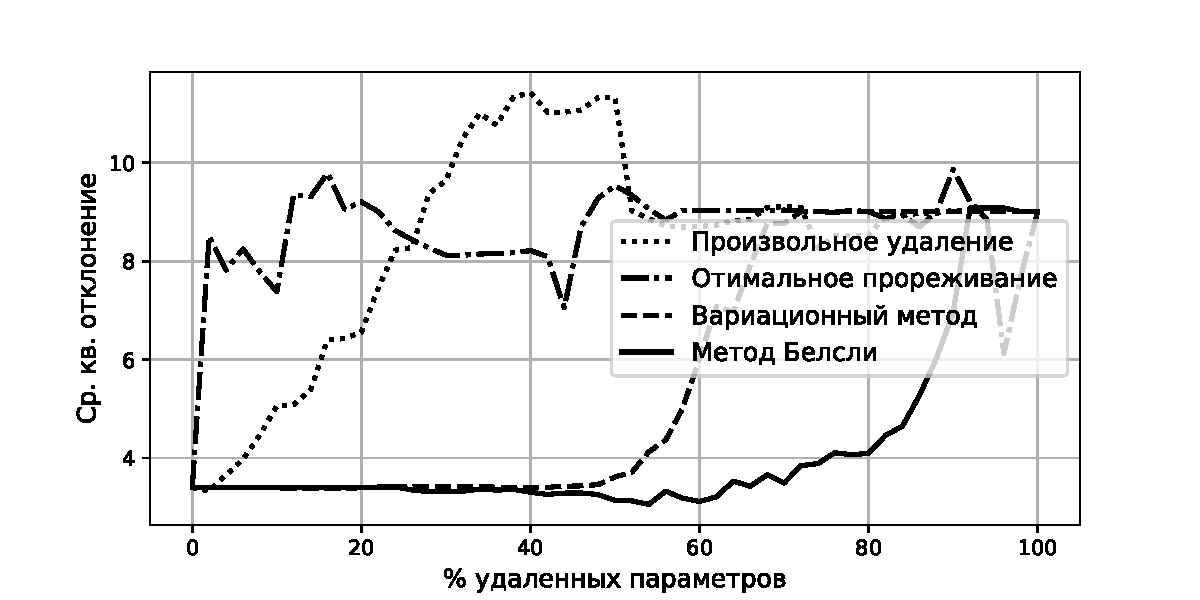
\includegraphics[width=0.8\textwidth]{plots/grabovoy/boston_all.pdf}\\
\caption{Качество прогноза при удаление параметров на выборке Boston}
\label{BostonAll}
\end{figure}



\begin{figure}[ht]\center
%\begin{subfigure}[а]{0.33\textwidth}
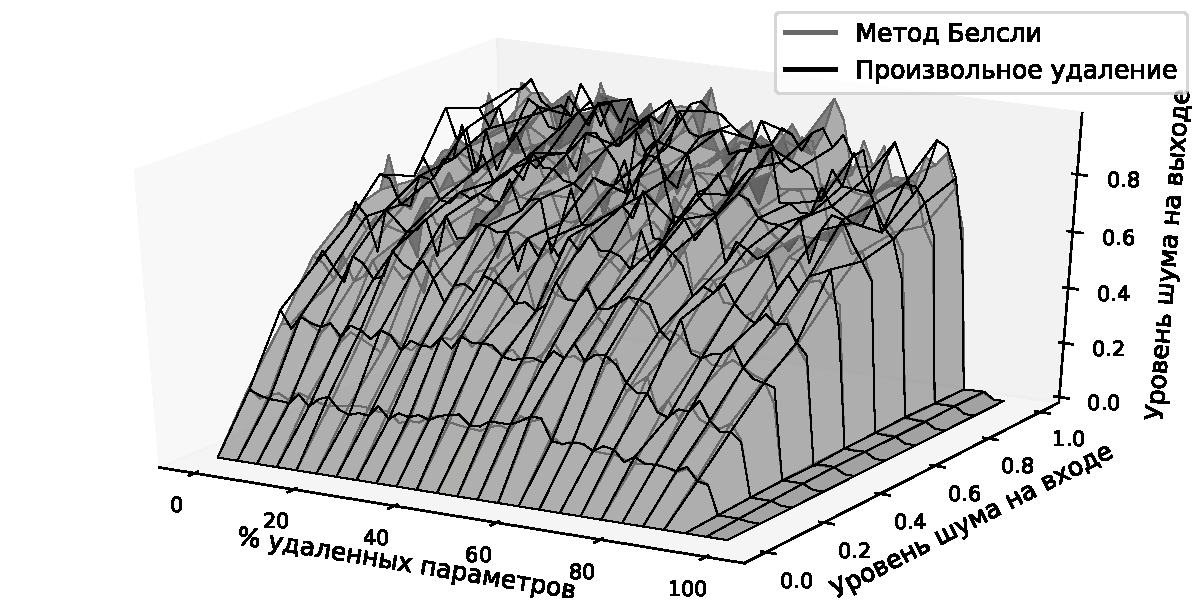
\includegraphics[width=0.33\textwidth]{plots/grabovoy/boston_random.pdf}
%\end{subfigure}
%\begin{subfigure}[б]{0.33\textwidth}
{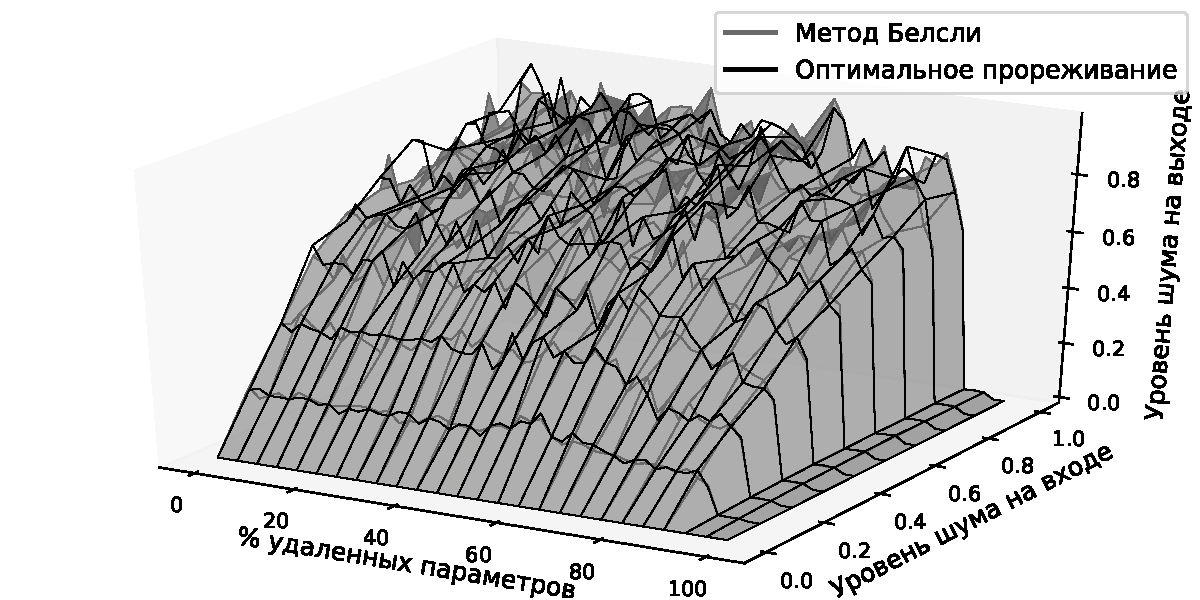
\includegraphics[width=0.33\textwidth]{plots/grabovoy/boston_obd.pdf}}
%\end{subfigure}
%\begin{subfigure}[в]{0.33\textwidth}
{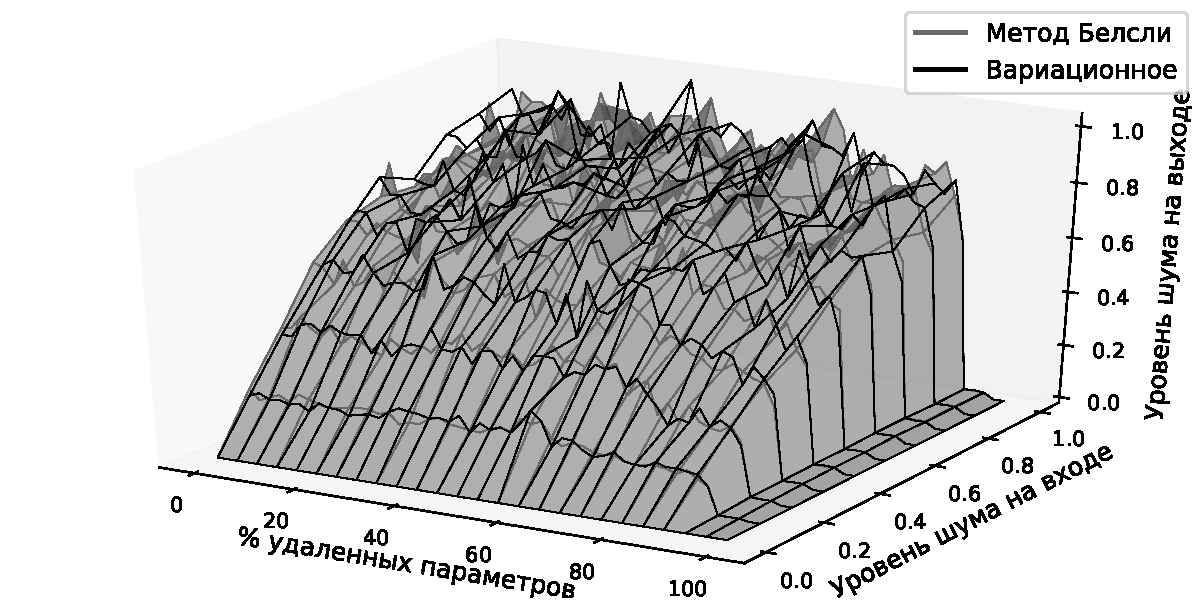
\includegraphics[width=0.33\textwidth]{plots/grabovoy/boston_var.pdf}}
%\end{subfigure}

%\subfigure[Оптимальное прореживание]{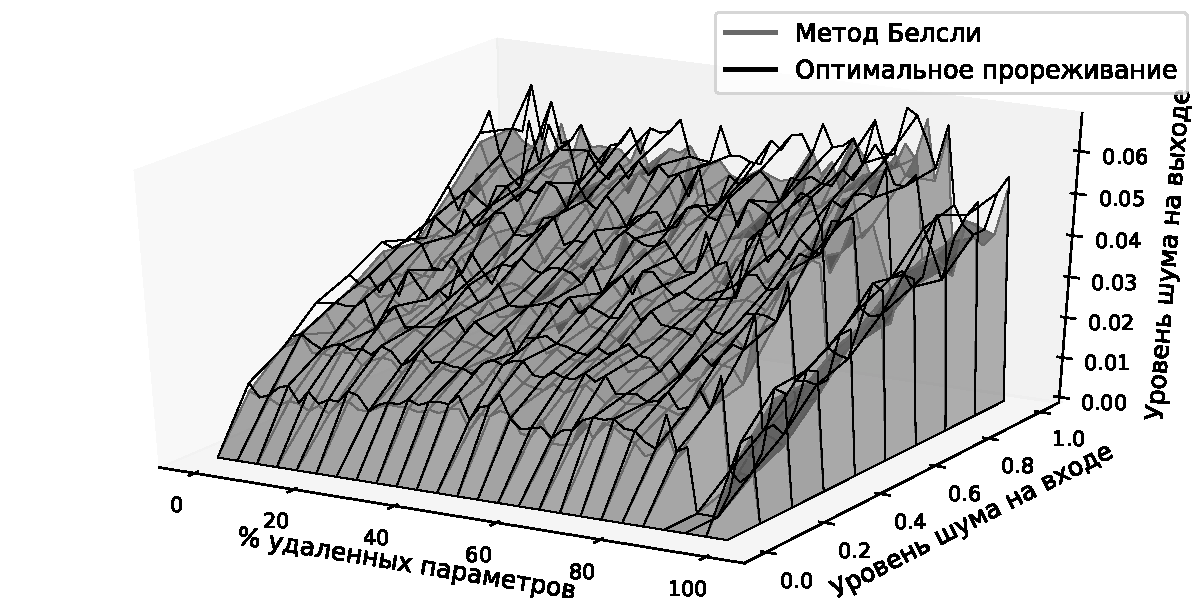
\includegraphics[width=0.5\textwidth]{plots/grabovoy/obd_noise_3d.pdf}}\\
%\subfigure[Вариационный метод]{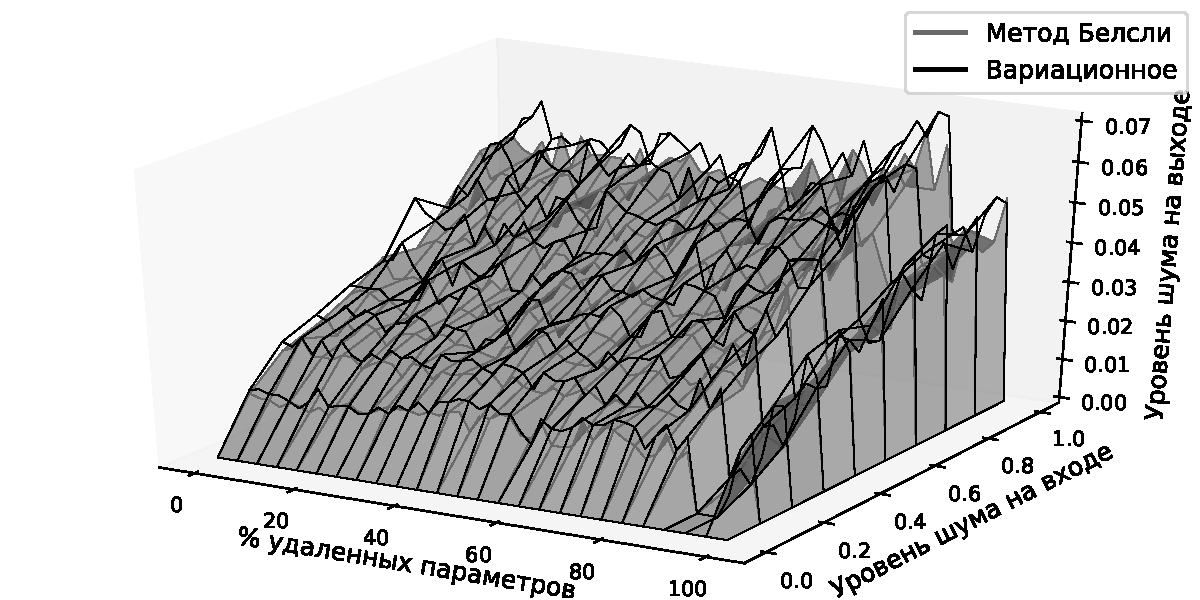
\includegraphics[width=0.5\textwidth]{plots/grabovoy/var_noise_3d.pdf}}
\caption{Влияние шума в начальных данных на шум выхода нейросети на выборке Boston: a --- Произвольное удаление параметров, б --- Оптимальное прореживание, в --- Вариационный метод}
\label{BostonNoise}
\end{figure}

На рис.~\ref{BostonAll} показано как меняется среднеквадратическое отклонение прогноза $\mathsf{R}_{\text{rg}}$ от точного ответа  при удалении параметров указанными методами. График показывает, что метод Белсли является более эффективным, чем другие методы, так-как позволяет удалить больше параметров нейросети без потери качества.

На рис.~\ref{BostonNoise} показаны поверхности изменения уровня шума ответов нейросети при изменении процента удаленных параметров и уровня шума входных данных для разных методов прореживания. График показывает, что уровень шума всех методов одинаковый, так-как поверхности всех методов находятся на одном уровне.


\textbf{Синтетические данные. } Рассмотрим нейроную сеть с 100 нейронами на входе и одним нейроном на выходе.

\begin{figure}[h!t]\center
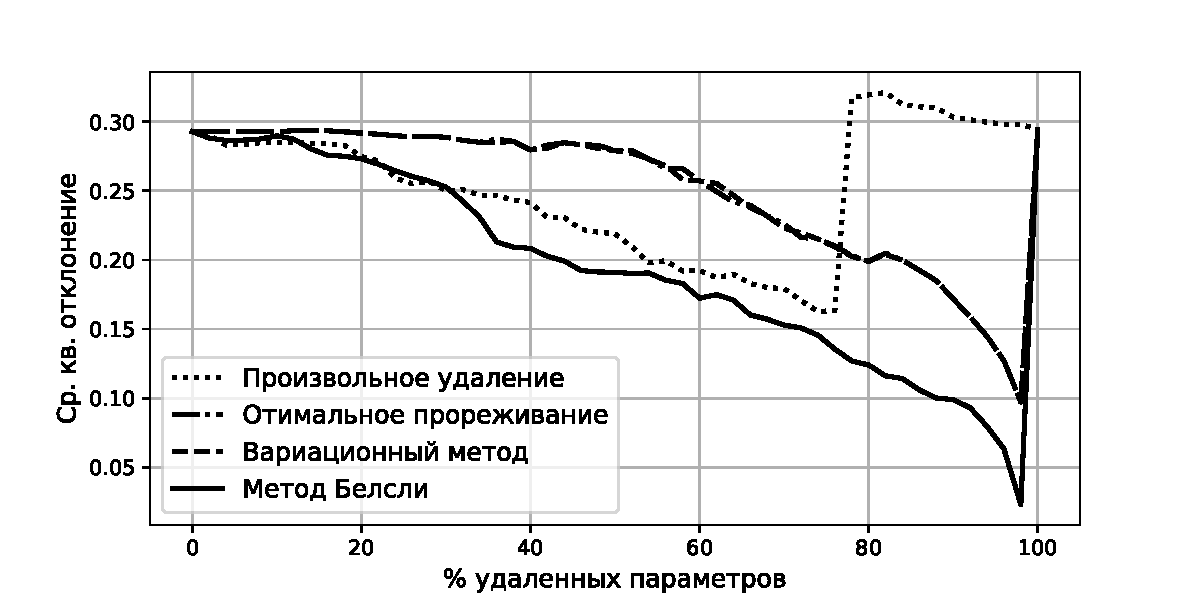
\includegraphics[width=0.8\textwidth]{plots/grabovoy/synt_all.pdf}\\
\caption{Качество прогноза при удаление параметров на синтетической выборке}
\label{Data1All}
\end{figure}

\begin{figure}[ht]\center
%\begin{subfigure}[а]{0.33\textwidth}
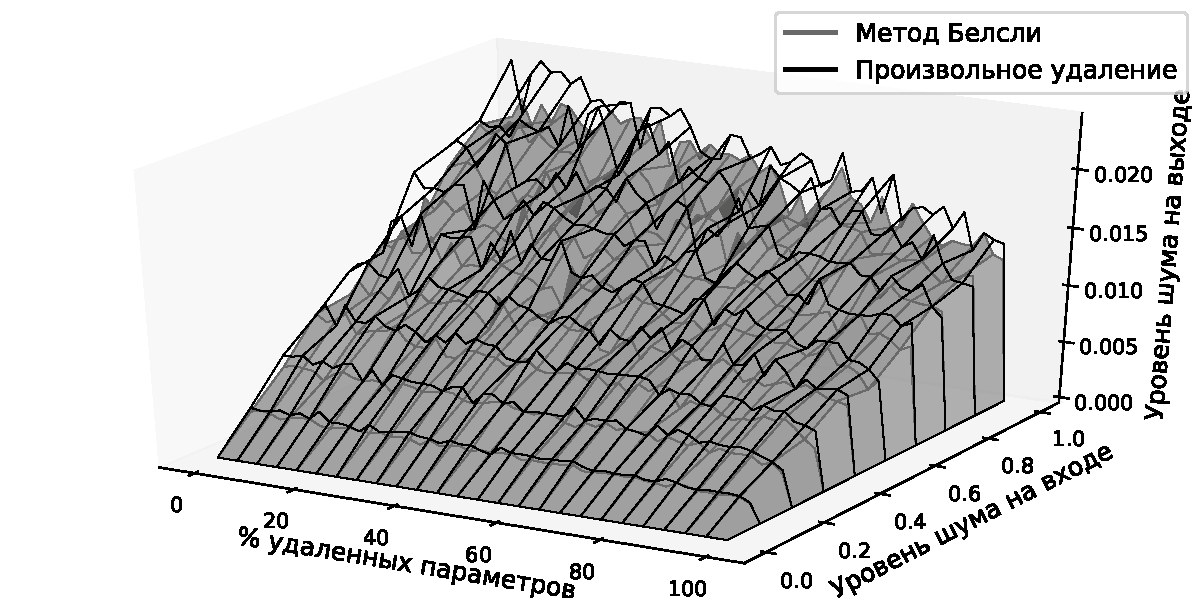
\includegraphics[width=0.33\textwidth]{plots/grabovoy/synt_random.pdf}
%\end{subfigure}
%\begin{subfigure}[б]{0.33\textwidth}
{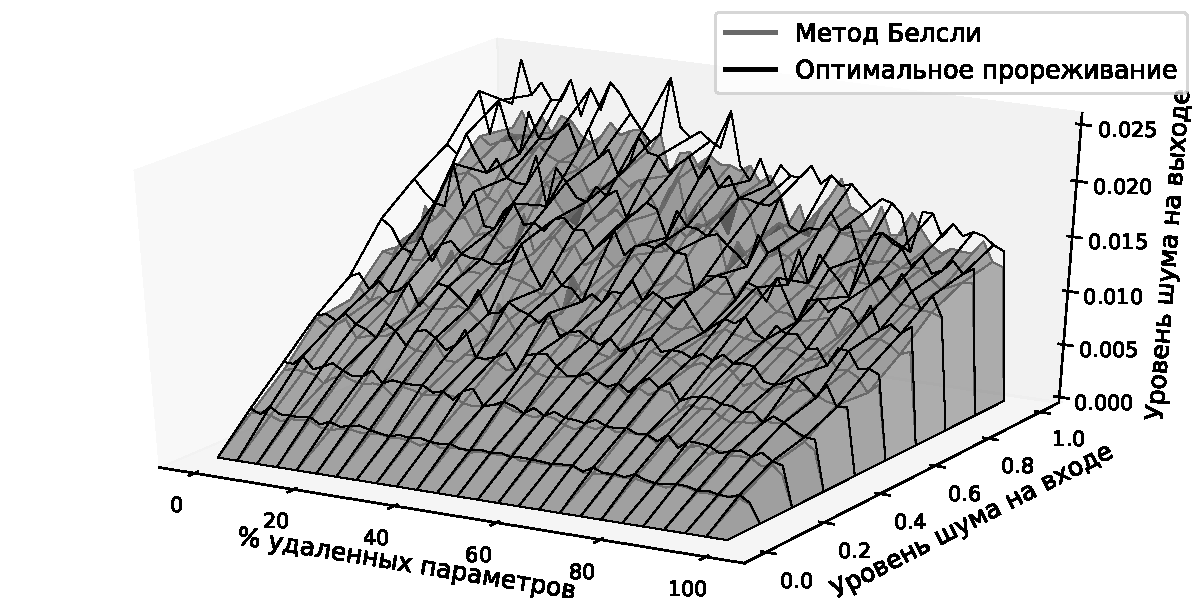
\includegraphics[width=0.33\textwidth]{plots/grabovoy/synt_obd.pdf}}
%\end{subfigure}
%\begin{subfigure}[в]{0.33\textwidth}
{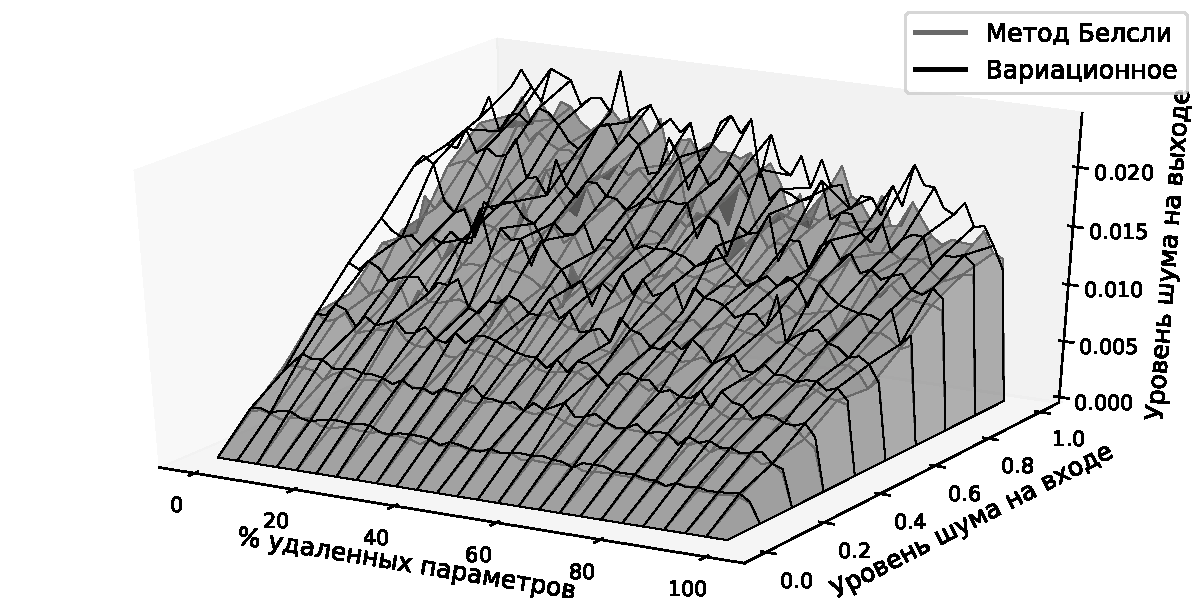
\includegraphics[width=0.33\textwidth]{plots/grabovoy/synt_var.pdf}}
%\end{subfigure}

%\subfigure[Оптимальное прореживание]{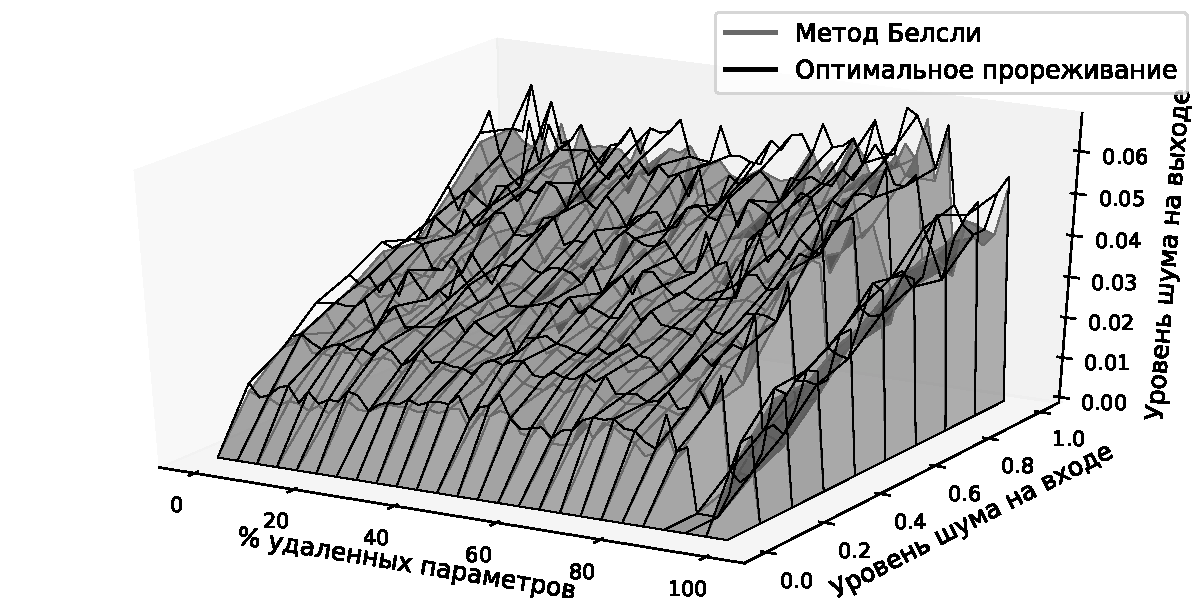
\includegraphics[width=0.5\textwidth]{plots/grabovoy/obd_noise_3d.pdf}}\\
%\subfigure[Вариационный метод]{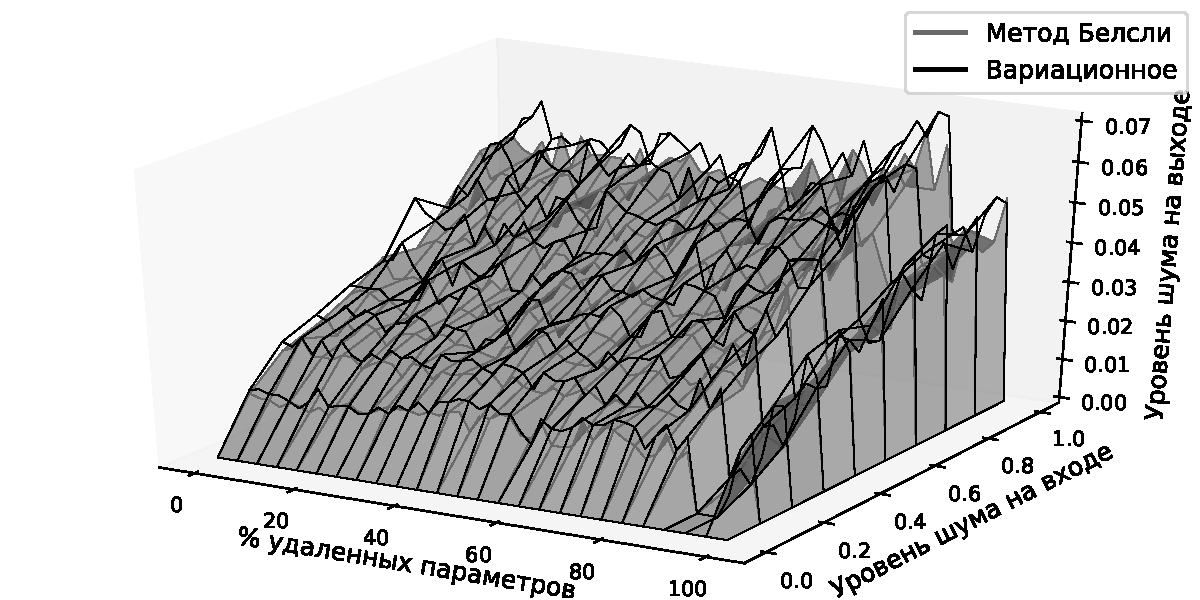
\includegraphics[width=0.5\textwidth]{plots/grabovoy/var_noise_3d.pdf}}
\caption{Влияние шума в начальных данных на шум выхода нейросети на выборке Boston: a --- Произвольное удаление параметров, б --- Оптимальное прореживание, в --- Вариационный метод}
\label{Data1Noise}
\end{figure}
На рис.~\ref{Data1All} показано как меняется среднеквадратическое отклонение прогноза от $\mathsf{R}_{\text{rg}}$ точного ответа при удалении параметров указанными методами. График показывает, что удаление параметров методом Белсли являеться более эффективным чем другие методы прореживания, так-как качество прогноза нейросети улучшается при удалении шумовых параметров.

На рис.~\ref{Data1Noise} показаны поверхности изменения уровня шума ответов нейросети при изменении процента удаленных параметров и уровня шума входных данных для разных методов прореживания. На графиках показано, что при удалении параметров нейросети методом Белсли шум меньше, чем при удалении параметров другими методами, так-как поверхность которая соответствует методу Белсли ниже других поверхностей.



